% Options for packages loaded elsewhere
\PassOptionsToPackage{unicode}{hyperref}
\PassOptionsToPackage{hyphens}{url}
%
\documentclass[
]{article}
\usepackage{lmodern}
\usepackage{amssymb,amsmath}
\usepackage{ifxetex,ifluatex}
\ifnum 0\ifxetex 1\fi\ifluatex 1\fi=0 % if pdftex
  \usepackage[T1]{fontenc}
  \usepackage[utf8]{inputenc}
  \usepackage{textcomp} % provide euro and other symbols
\else % if luatex or xetex
  \usepackage{unicode-math}
  \defaultfontfeatures{Scale=MatchLowercase}
  \defaultfontfeatures[\rmfamily]{Ligatures=TeX,Scale=1}
\fi
% Use upquote if available, for straight quotes in verbatim environments
\IfFileExists{upquote.sty}{\usepackage{upquote}}{}
\IfFileExists{microtype.sty}{% use microtype if available
  \usepackage[]{microtype}
  \UseMicrotypeSet[protrusion]{basicmath} % disable protrusion for tt fonts
}{}
\makeatletter
\@ifundefined{KOMAClassName}{% if non-KOMA class
  \IfFileExists{parskip.sty}{%
    \usepackage{parskip}
  }{% else
    \setlength{\parindent}{0pt}
    \setlength{\parskip}{6pt plus 2pt minus 1pt}}
}{% if KOMA class
  \KOMAoptions{parskip=half}}
\makeatother
\usepackage{xcolor}
\IfFileExists{xurl.sty}{\usepackage{xurl}}{} % add URL line breaks if available
\IfFileExists{bookmark.sty}{\usepackage{bookmark}}{\usepackage{hyperref}}
\hypersetup{
  pdftitle={STAT461 HW7},
  pdfauthor={Xiangyu Ren},
  hidelinks,
  pdfcreator={LaTeX via pandoc}}
\urlstyle{same} % disable monospaced font for URLs
\usepackage[margin=1in]{geometry}
\usepackage{color}
\usepackage{fancyvrb}
\newcommand{\VerbBar}{|}
\newcommand{\VERB}{\Verb[commandchars=\\\{\}]}
\DefineVerbatimEnvironment{Highlighting}{Verbatim}{commandchars=\\\{\}}
% Add ',fontsize=\small' for more characters per line
\usepackage{framed}
\definecolor{shadecolor}{RGB}{248,248,248}
\newenvironment{Shaded}{\begin{snugshade}}{\end{snugshade}}
\newcommand{\AlertTok}[1]{\textcolor[rgb]{0.94,0.16,0.16}{#1}}
\newcommand{\AnnotationTok}[1]{\textcolor[rgb]{0.56,0.35,0.01}{\textbf{\textit{#1}}}}
\newcommand{\AttributeTok}[1]{\textcolor[rgb]{0.77,0.63,0.00}{#1}}
\newcommand{\BaseNTok}[1]{\textcolor[rgb]{0.00,0.00,0.81}{#1}}
\newcommand{\BuiltInTok}[1]{#1}
\newcommand{\CharTok}[1]{\textcolor[rgb]{0.31,0.60,0.02}{#1}}
\newcommand{\CommentTok}[1]{\textcolor[rgb]{0.56,0.35,0.01}{\textit{#1}}}
\newcommand{\CommentVarTok}[1]{\textcolor[rgb]{0.56,0.35,0.01}{\textbf{\textit{#1}}}}
\newcommand{\ConstantTok}[1]{\textcolor[rgb]{0.00,0.00,0.00}{#1}}
\newcommand{\ControlFlowTok}[1]{\textcolor[rgb]{0.13,0.29,0.53}{\textbf{#1}}}
\newcommand{\DataTypeTok}[1]{\textcolor[rgb]{0.13,0.29,0.53}{#1}}
\newcommand{\DecValTok}[1]{\textcolor[rgb]{0.00,0.00,0.81}{#1}}
\newcommand{\DocumentationTok}[1]{\textcolor[rgb]{0.56,0.35,0.01}{\textbf{\textit{#1}}}}
\newcommand{\ErrorTok}[1]{\textcolor[rgb]{0.64,0.00,0.00}{\textbf{#1}}}
\newcommand{\ExtensionTok}[1]{#1}
\newcommand{\FloatTok}[1]{\textcolor[rgb]{0.00,0.00,0.81}{#1}}
\newcommand{\FunctionTok}[1]{\textcolor[rgb]{0.00,0.00,0.00}{#1}}
\newcommand{\ImportTok}[1]{#1}
\newcommand{\InformationTok}[1]{\textcolor[rgb]{0.56,0.35,0.01}{\textbf{\textit{#1}}}}
\newcommand{\KeywordTok}[1]{\textcolor[rgb]{0.13,0.29,0.53}{\textbf{#1}}}
\newcommand{\NormalTok}[1]{#1}
\newcommand{\OperatorTok}[1]{\textcolor[rgb]{0.81,0.36,0.00}{\textbf{#1}}}
\newcommand{\OtherTok}[1]{\textcolor[rgb]{0.56,0.35,0.01}{#1}}
\newcommand{\PreprocessorTok}[1]{\textcolor[rgb]{0.56,0.35,0.01}{\textit{#1}}}
\newcommand{\RegionMarkerTok}[1]{#1}
\newcommand{\SpecialCharTok}[1]{\textcolor[rgb]{0.00,0.00,0.00}{#1}}
\newcommand{\SpecialStringTok}[1]{\textcolor[rgb]{0.31,0.60,0.02}{#1}}
\newcommand{\StringTok}[1]{\textcolor[rgb]{0.31,0.60,0.02}{#1}}
\newcommand{\VariableTok}[1]{\textcolor[rgb]{0.00,0.00,0.00}{#1}}
\newcommand{\VerbatimStringTok}[1]{\textcolor[rgb]{0.31,0.60,0.02}{#1}}
\newcommand{\WarningTok}[1]{\textcolor[rgb]{0.56,0.35,0.01}{\textbf{\textit{#1}}}}
\usepackage{graphicx,grffile}
\makeatletter
\def\maxwidth{\ifdim\Gin@nat@width>\linewidth\linewidth\else\Gin@nat@width\fi}
\def\maxheight{\ifdim\Gin@nat@height>\textheight\textheight\else\Gin@nat@height\fi}
\makeatother
% Scale images if necessary, so that they will not overflow the page
% margins by default, and it is still possible to overwrite the defaults
% using explicit options in \includegraphics[width, height, ...]{}
\setkeys{Gin}{width=\maxwidth,height=\maxheight,keepaspectratio}
% Set default figure placement to htbp
\makeatletter
\def\fps@figure{htbp}
\makeatother
\setlength{\emergencystretch}{3em} % prevent overfull lines
\providecommand{\tightlist}{%
  \setlength{\itemsep}{0pt}\setlength{\parskip}{0pt}}
\setcounter{secnumdepth}{-\maxdimen} % remove section numbering

\title{STAT461 HW7}
\author{Xiangyu Ren}
\date{10/23/2020}

\begin{document}
\maketitle

\hypertarget{problem-1.-your-homework-will-consider-an-experiment-on-battery-life-for-different-types-and-brands-of-battery.-two-brands-a-name-brand-and-a-generic-brand-of-two-types-alkaline-and-heavy-duty-of-batteries-were-tested-to-see-how-long-they-could-run-continuously.-this-results-in-four-categories-alkname-is-for-name-brand-alkaline-batteries-alkgen-is-for-generic-alkaline-batteries-hdname-is-for-heavy-duty-name-brand-batteries-and-hdgen-is-for-generic-heavy-duty-batteries.-four-batteries-of-each-type-were-tested-and-the-times-to-battery-failure-are-recorded-as-below.-use-the-code-below-to-read-in-the-data}{%
\paragraph{Problem 1. Your homework will consider an experiment on
battery life for different types and brands of battery. Two brands (a
name brand and a generic brand) of two types (Alkaline and ``Heavy
Duty'') of batteries were tested to see how long they could run
continuously. This results in four categories, AlkName is for name-brand
alkaline batteries, AlkGen is for generic alkaline batteries, HDName is
for heavy duty name-brand batteries, and HDGen is for generic heavy duty
batteries. Four batteries of each type were tested and the times to
battery failure are recorded as below. Use the code below to read in the
data:}\label{problem-1.-your-homework-will-consider-an-experiment-on-battery-life-for-different-types-and-brands-of-battery.-two-brands-a-name-brand-and-a-generic-brand-of-two-types-alkaline-and-heavy-duty-of-batteries-were-tested-to-see-how-long-they-could-run-continuously.-this-results-in-four-categories-alkname-is-for-name-brand-alkaline-batteries-alkgen-is-for-generic-alkaline-batteries-hdname-is-for-heavy-duty-name-brand-batteries-and-hdgen-is-for-generic-heavy-duty-batteries.-four-batteries-of-each-type-were-tested-and-the-times-to-battery-failure-are-recorded-as-below.-use-the-code-below-to-read-in-the-data}}

\begin{Shaded}
\begin{Highlighting}[]
\NormalTok{type<-}\KeywordTok{c}\NormalTok{(}\StringTok{"AlkName"}\NormalTok{,}\StringTok{"AlkName"}\NormalTok{,}\StringTok{"AlkName"}\NormalTok{,}\StringTok{"AlkName"}\NormalTok{,}\StringTok{"AlkGen"}\NormalTok{,}\StringTok{"AlkGen"}\NormalTok{,}\StringTok{"AlkGen"}\NormalTok{,}\StringTok{"AlkGen"}\NormalTok{,}
\StringTok{"HDName"}\NormalTok{,}\StringTok{"HDName"}\NormalTok{,}\StringTok{"HDName"}\NormalTok{,}\StringTok{"HDName"}\NormalTok{,}\StringTok{"HDGen"}\NormalTok{,}\StringTok{"HDGen"}\NormalTok{,}\StringTok{"HDGen"}\NormalTok{,}\StringTok{"HDGen"}\NormalTok{)}
\NormalTok{life<-}\KeywordTok{c}\NormalTok{(}\FloatTok{100.668}\NormalTok{, }\FloatTok{77.734}\NormalTok{,}\FloatTok{79.210}\NormalTok{,}\FloatTok{95.063}\NormalTok{,}\FloatTok{206.880}\NormalTok{,}\FloatTok{153.347}\NormalTok{,}\FloatTok{165.980}\NormalTok{,}\FloatTok{196.000}\NormalTok{,}
\FloatTok{14.951}\NormalTok{,}\FloatTok{18.063}\NormalTok{,}\FloatTok{11.111}\NormalTok{,}\FloatTok{12.840}\NormalTok{,}\FloatTok{15.340}\NormalTok{,}\FloatTok{22.090}\NormalTok{,}\FloatTok{15.734}\NormalTok{, }\FloatTok{14.440}\NormalTok{)}
\NormalTok{batt<-}\KeywordTok{data.frame}\NormalTok{(}\DataTypeTok{type=}\NormalTok{type, }\DataTypeTok{life=}\NormalTok{life)}
\end{Highlighting}
\end{Shaded}

\hypertarget{plot-the-data.}{%
\paragraph{1. Plot the data.}\label{plot-the-data.}}

\begin{Shaded}
\begin{Highlighting}[]
\KeywordTok{boxplot}\NormalTok{(life }\OperatorTok{~}\StringTok{ }\NormalTok{type, }\DataTypeTok{data =}\NormalTok{ batt)}
\end{Highlighting}
\end{Shaded}

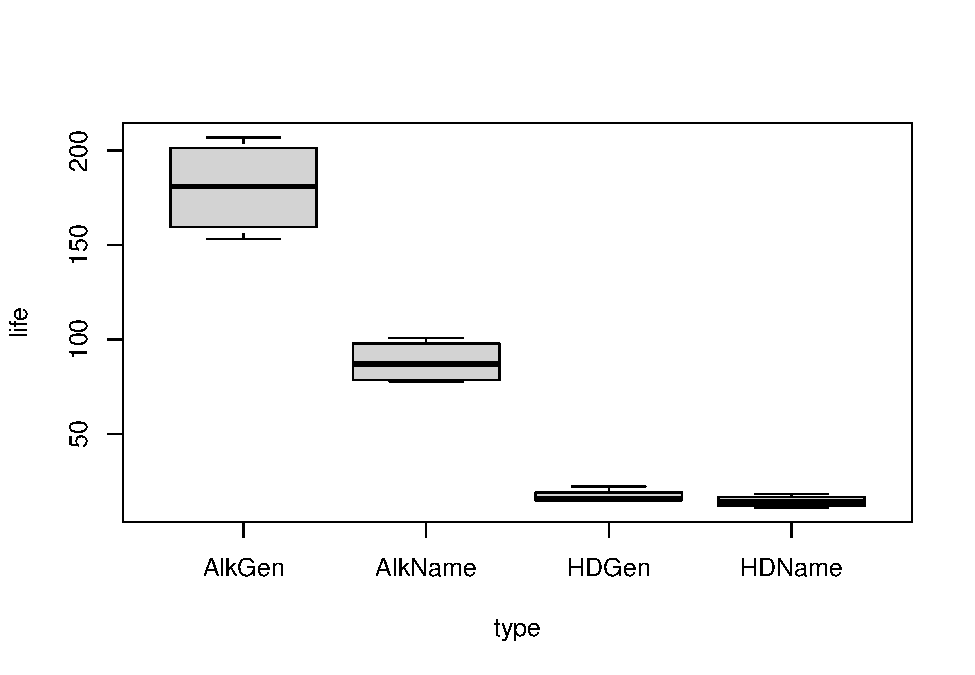
\includegraphics{HW7_XiangyuRen_files/figure-latex/unnamed-chunk-2-1.pdf}

\hypertarget{for-the-battery-data-do-the-following}{%
\paragraph{2. For the battery data, do the
following:}\label{for-the-battery-data-do-the-following}}

\hypertarget{a-write-out-the-one-way-anova-model-for-this-data.}{%
\paragraph{(a) Write out the one-way ANOVA model for this
data.}\label{a-write-out-the-one-way-anova-model-for-this-data.}}

\(Y_{it}=µ+τ_{i}+\epsilon_{it}\), \(i=AN,AG,HN,HG\) \(t=1,2,3,4\)
\[\epsilon_{it}\overset{\text{iid}}{\sim}N(0,\sigma^2)\]

\hypertarget{show-residual-plots-for-this-model.-are-the-residuals-approximately-normal-justify-your-answer.}{%
\paragraph{Show residual plots for this model. Are the residuals
approximately normal? Justify your
answer.}\label{show-residual-plots-for-this-model.-are-the-residuals-approximately-normal-justify-your-answer.}}

\begin{Shaded}
\begin{Highlighting}[]
\NormalTok{model1 =}\StringTok{ }\KeywordTok{aov}\NormalTok{(life }\OperatorTok{~}\StringTok{ }\NormalTok{type, }\DataTypeTok{data =}\NormalTok{ batt)}
\KeywordTok{plot}\NormalTok{(model1, }\DataTypeTok{which =} \KeywordTok{c}\NormalTok{(}\DecValTok{1}\NormalTok{, }\DecValTok{2}\NormalTok{))}
\end{Highlighting}
\end{Shaded}

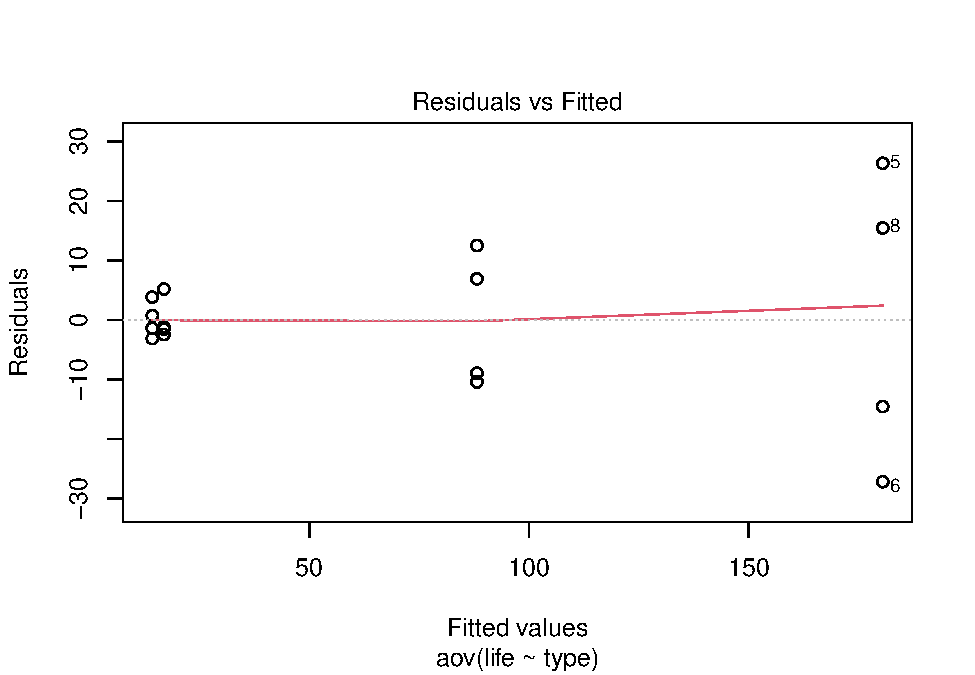
\includegraphics{HW7_XiangyuRen_files/figure-latex/unnamed-chunk-3-1.pdf}
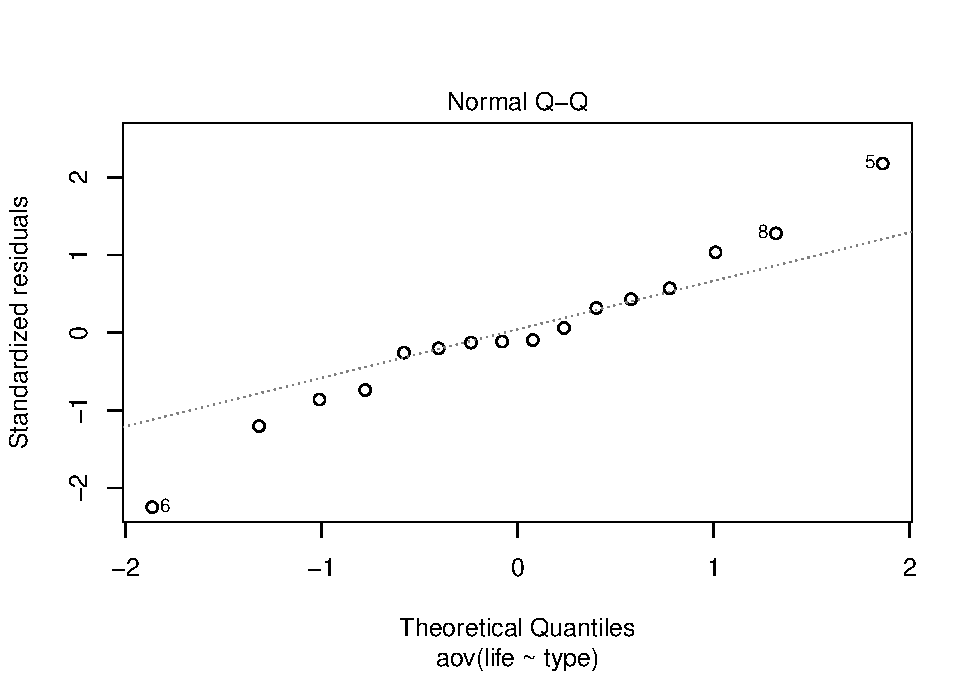
\includegraphics{HW7_XiangyuRen_files/figure-latex/unnamed-chunk-3-2.pdf}

In the first plot, it seems like the abline is a straight line, and in
the QQ plot, all the observations are like having linear relation, thus
we say the residuals are approximately normal.

\hypertarget{c-is-the-assumption-of-constant-error-variance-among-treatments-justified-explain-your-answer.}{%
\paragraph{(c) Is the assumption of constant error variance among
treatments justified? Explain your
answer.}\label{c-is-the-assumption-of-constant-error-variance-among-treatments-justified-explain-your-answer.}}

\begin{Shaded}
\begin{Highlighting}[]
\NormalTok{v1 =}\StringTok{ }\KeywordTok{var}\NormalTok{(life[type}\OperatorTok{==}\StringTok{"AlkName"}\NormalTok{])}
\NormalTok{v2 =}\StringTok{ }\KeywordTok{var}\NormalTok{(life[type}\OperatorTok{==}\StringTok{"AlkGen"}\NormalTok{])}
\NormalTok{v3 =}\StringTok{ }\KeywordTok{var}\NormalTok{(life[type}\OperatorTok{==}\StringTok{"HDName"}\NormalTok{])}
\NormalTok{v4 =}\StringTok{ }\KeywordTok{var}\NormalTok{(life[type}\OperatorTok{==}\StringTok{"HDGen"}\NormalTok{])}
\NormalTok{v1;v2;v3;v4;v2}\OperatorTok{/}\NormalTok{v3}
\end{Highlighting}
\end{Shaded}

\begin{verbatim}
## [1] 130.9684
\end{verbatim}

\begin{verbatim}
## [1] 628.0865
\end{verbatim}

\begin{verbatim}
## [1] 8.957162
\end{verbatim}

\begin{verbatim}
## [1] 12.26028
\end{verbatim}

\begin{verbatim}
## [1] 70.12115
\end{verbatim}

\end{document}
